\documentclass[a4paper, 11pt]{article}          % Paper and font size
\usepackage[ngerman,english]{babel}               % Language setting

% Set margins
\usepackage[top=2.5cm,bottom=2.5cm,left=2cm,right=2cm,marginparwidth=1.75cm]{geometry}

% Load useful packages
\usepackage{graphicx}                           % Graphics
\usepackage{subcaption}                         % Sub-figures / grids of plots
\graphicspath{{figures/}}                       % Look for images in report/figures/
\usepackage{amsmath}                            % Math
\usepackage{xcolor}                             % Link color
\definecolor{custom-blue}{RGB}{0,99,166}
\usepackage{hyperref}
\hypersetup{colorlinks=true, allcolors=custom-blue}
\usepackage[default]{sourcesanspro}                % Load font
\usepackage[T1]{fontenc}                        % Special characters
\usepackage{fancyhdr}
\usepackage{float}

\usepackage{amssymb}
\usepackage{booktabs}                           % Rules used by the generated tables in tables/

\usepackage{tikz}
\usepackage{pdflscape}                          % Landscape pages for wide code listings

% Code listings (used in the appendix) -----------------------------------
\usepackage{listings}
\definecolor{code-comment}{RGB}{110,110,110}
\definecolor{code-keyword}{RGB}{0,70,130}
\definecolor{code-string}{RGB}{100,60,0}
\definecolor{code-bg}{RGB}{247,247,247}

\lstdefinestyle{pythonstyle}{
    language=Python,
    backgroundcolor=\color{code-bg},
    basicstyle=\ttfamily\scriptsize,
    keywordstyle=\color{code-keyword}\bfseries,
    commentstyle=\color{code-comment}\itshape,
    stringstyle=\color{code-string},
    numbers=left,
    numberstyle=\tiny\color{code-comment},
    numbersep=8pt,
    frame=single,
    rulecolor=\color{black!30},
    breaklines=true,
    breakatwhitespace=false,
    breakindent=0pt,
    postbreak=\mbox{\textcolor{code-comment}{$\hookrightarrow$}\space},
    tabsize=4,
    showstringspaces=false,
    captionpos=b,
    xleftmargin=1.5em,
    framexleftmargin=1.2em
}
% Load header, footer package

\usepackage{lastpage}                           % Footer note
\usepackage{lipsum}                             % For dummy text

\pagestyle{myheadings}                          % Own header
\pagestyle{fancy}                               % Own style
\fancyhf{}                                      % Clear header, footer

\setlength{\headheight}{30pt}                   % Set header hight
\renewcommand{\headrulewidth}{0.5pt}            % Top line
\renewcommand{\footrulewidth}{0.5pt}            % Bottom line

\fancyhead[L]{
\includegraphics[width=3cm]{univienna-logo.eps}} % Header left
\fancyhead[C]{DMC Project Report }                                 % Header center
\fancyhead[R]{University of Vienna}             % Header right
                             % Footer center
\fancyfoot[R]{\thepage/\pageref{LastPage}}      % Footer right

\usepackage{parskip}

\usepackage[
    natbib=true,
    backend=biber,
    sorting=none
]{biblatex}
\addbibresource{report.bib}

%% CONTACT: zid.univie.ac.at
%% KONTAKT: zid.univie.ac.at


%%% Begin document %%%
\begin{document}

    \begin{figure}                                  % Include Logo
        \flushleft
        
\includegraphics[width=0.4\textwidth]{univienna-logo.eps}\label{fig:logo}
    \end{figure}

% Set title, author, date
    \title{Variational Monte Carlo for solving the Schrödinger Equation for simple potentials}
    \author{Valentin Mayer | a12213346@unet.univie.ac.at}
    \date{\today{}, Vienna}

    \maketitle                                      % Include contents
    \tableofcontents

    \newpage
    \section {Introduction and problem description}
    This report documents the implementation of a variational Monte Carlo (VMC) approach to solving the Schödinger Equation for simple potentials up to the helium atom. The solution follows the methods described in Chapter 12 of \cite{Thijssen2007} The source code is available on Github at the following link: \href{https://github.com/lordVelisch/variational-monte-carlo}{Github} and all calculations are reproducible from this project. Some of the most important parts of the source code are also shown in the appendix.

    \section{Methods}

    The goal of this project is to calculate the ground state energies of a 1D harmonic oscillator, the hydrogen atom and the helium atom in 3 dimensions using the Schrödinger equation:

    \begin{equation}\label{eq:schrödinger}
        \hat{H} |\psi_n \rangle = E_n |\psi_n \rangle
    \end{equation}

    where $|\psi \rangle$ is the wave function in state $n$, $\hat{H}$ is the Hamiltonian and $E_n$ is the corresponding energy. By multiplying with $\langle \psi |$ from the left and rearranging we end up with the equation:

    \begin{equation}\label{eq:H_expectation}
        \frac{\langle \psi | H|\psi \rangle}{\langle \psi | \psi \rangle} = \frac{\int \psi(r) (\hat{H}\psi(r)) dr}{\int \psi^2(r) dr} =  \langle H \rangle_{\psi}
    \end{equation}

    Here the dirac notation is written using the explicit integrals and $|\psi \rangle$ is always used as a shorthand for $|\psi(r)\rangle$ where r is the position in space. We assume $\psi$ to be real. Ritz theorem says that for any trial wavefunction $\psi_T$ equation $\langle H \rangle_{\psi_T}$ must always be greater or equal to the ground state $E_0$. This means that minimizing $\eqref{eq:H_expectation}$ is equivalent to finding the correct ground state.

    There are multiple challenges in calculating the integrals as they are written here. The exact form of $\psi$ is obviously not known, so a parametrized trial wavefunction $\psi_T(\alpha)$ has to be used where by varying the set of parameters $\alpha$ the true wavefunction can be recovered as well as possible. One example would be to use plane waves $\psi_T(\alpha, r) = e^{\alpha r}$. The more general $\psi_T$ the higher the chances to recover something close to the true form of the wavefunction, but this also increases the amount of parameters and therefore the search space for minimization. Also, depending on the choice of trial wavefunctions the integrals might not be analytically solvable anymore so numerical methods have to be used. However, $\psi$ depends on the position of all particles involved in the simulation, which leads to a very high dimensional integral even for small systems. Simulating carbon for example already includes 6 electrons, which in 3 dimensions leads to 18 integration variables and that is already with the nucleus to be considered as classical.

    Using direct numerical integration methods on a fixed grid lead to large errors in higher dimension. It can be shown that for any quadrature rule $Q_n(f)$ of the form $Q_n(f)=\sum_{j=1}^n w_j f(x_j)$ with $w_j$ the weights and $x_j$ the nodes, and $n$ is the order for a $d$-dimensional integral $I_d(f)$ there exists a lower bound on the error:

    \begin{equation*}
        |Q_n(f) - I_d(f)| \geq \frac{k}{n^{r/d}}
    \end{equation*}

    where $k > 0$ is a constant and $r$ is also limited. This implies that the lower bound on the error grows with the number of dimensions. The systems calculated here a small enough to be calculated without any significant error but this result implies that generally direct integration is unfeasible for the quantum mechanical systems.

    Instead, monte carlo integration is used, which has no dependence on the dimensions for its error estimation. To make use of it we define the local energy as

    \begin{equation}\label{eq:local_energy}
        E_L(r) = \frac{\hat{H}\psi_T(r)}{\psi_T(r)}
    \end{equation}

    as a direct consequence of the stationary schrödinger equation \eqref{eq:schrödinger}. This way equation \eqref{eq:H_expectation} can be rewritten as

    \begin{equation}\label{eq:H_expectation_as_expectation_value}
        \langle E_L \rangle_{\psi_T^2} = \frac{\int \psi_T^2(r) E_L(r) dr}{\int \psi_T^2(r) dr}
    \end{equation}

    Which can be solved by Monte Carlo integration by calculating the mean of $E_L(r_i)$ where $r_i$ is drawn from the normalized probability density:

    \begin{equation*}
        p(r) = \frac{\psi_T^2(r)}{\int \psi_T^2(r) dr}
    \end{equation*}

    % todo: in reality \psi and not \psi^2 is used. why can I do that?

    Note that all integrals mentioned in this report go over the whole $\mathbb{R}^3$ as every particle can theoretically exist in any point in space. To actually generate samples from $p(r)$ the Metropolis-Hastings algorithm is used which makes the acceptance criterion

    \begin{equation*}
        p_{acc}(r \rightarrow r_{proposed}) = \min \left\{ 1, \frac{\psi_T^2(r_{proposed})}{\psi_T^2(r)} \right\}
    \end{equation*}

    This works for a symmetric generation probability, which is achieved here by proposing a new step using the following procedure: Starting from random initial positions for all particles with every component drawn from a uniform distribution $U(-1,1)$ on every move a disposition for all particles of the simulation is proposed inside a box around the current $r$ with length $\delta$ in all directions.

    \begin{equation*}
        r_{proposed}^j = r^j+ (\frac{1}{2}-\xi)\delta
    \end{equation*}

    where $j$ is the component in on direction and $\xi$ is a random number drawn from the uniform distribution $U(0,1)$.

    Usually the variance of the observable in a monte carlo simulation is mainly relevant for calculating the statistical error that comes from sampling finite points. However, in this simulation it holds an even more relevant role. The way $E_L(r)$ is constructed, implies that if $\psi_T(\alpha, r) = \psi(r)$ then

    \begin{equation*}
        E_L(r) = \frac{\hat{H} \psi(r)}{\psi(r)} \Rightarrow E_L \psi(r) = \hat{H} \psi(r)
    \end{equation*}

    $E_L$ is the exact eigenvalue of wavefunction $\psi$ and becomes a constant, leaving the variance exactly 0, and therefore also only needing sample to calculate the correct result.

    This opens the possibility to a different minimization scheme. Instead of minimizing the expectation value of $\langle H \rangle_\psi$ we could also try minimizing the variance of $\langle E_L(r) \rangle_{\psi^2}$. For this educational exercise however, just a simple fixed grid search is used for the minimization.

    \section{Results}

    \subsection{Harmonic oscillator}
    The harmonic oscillator in 1D has the Hamiltonian

    \begin{equation}\label{eq:hamiltonian_HO}
        H_{HO} = -\frac{1}{2}\frac{d^2}{dr^2}+\frac{1}{2}r^2
    \end{equation}

    Note that for calculations dimensionless units where used. The local energy function for this and the following systems was calculated using \eqref{eq:local_energy} and the resulting equations can be found in \cite{Thijssen2007}. The trial function used in this simulation is

    \begin{equation*}
        \psi_T(\alpha, r)=e^{-\alpha r^2}
    \end{equation*}

    Using Monte Carlo integration with the length of the displacement box set to $\delta=0.8$ the results are shown in table \ref{tab:harmonic_oscillator} and plotted in figure \ref{fig:harmonic_oscillator}.

    \begin{figure}[H]
        \centering
        \begin{minipage}[c]{0.36\textwidth}
            \centering
            \begin{tabular}{ccc}
\toprule
$\alpha$ & $\langle E \rangle$ & $\mathrm{var}(\langle E \rangle)$ \\
\midrule
$0.400$ & $0.51278$ & $0.02543$ \\
$0.450$ & $0.50282$ & $0.00558$ \\
$0.500$ & $0.50000$ & $0.00000$ \\
$0.550$ & $0.50209$ & $0.00458$ \\
$0.600$ & $0.50806$ & $0.01683$ \\
\bottomrule
\end{tabular}

            \captionof{table}{VMC energies for the harmonic oscillator at the $\alpha$ values in the book, Table 12.1 of \cite{Thijssen2007}.}
            \label{tab:harmonic_oscillator}
        \end{minipage}\hfill
        \begin{minipage}[c]{0.60\textwidth}
            \centering
            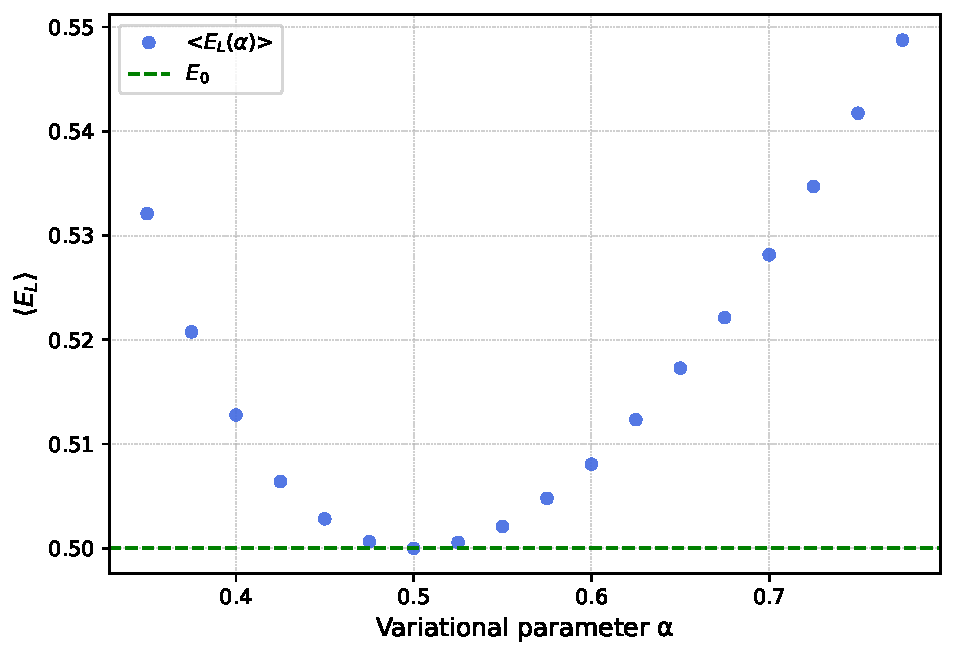
\includegraphics[width=\linewidth]{harmonic_oscillator.pdf}
            \caption{$\langle E_L \rangle$ over the full $\alpha$ grid, with the exact ground state energy $E_0 = 1/2$ as a reference. The x-axis shows the parameter $\alpha$ of the trial wavefunction $\psi_T$. The y-axis shows the expectation value calculated using the VMC approach.}
            \label{fig:harmonic_oscillator}
        \end{minipage}
    \end{figure}

    The exact wavefunction for the harmonic oscillator is $\psi(r)=e^{-r^2/2}$, which lies in the variational subspace of $\psi_T(\alpha, r)$ at $\alpha=0.5$. This expectation is confirmed in the results and can be seen at the minimum of the wavefunction at exactly the correct value $\alpha=0.5$ and a variance of 0 at that point. The numbers also agree with the reference \cite{Thijssen2007}.


    \subsection{Hydrogen atom}

    The hydrogen is treated here as a 3D problem which makes the Hamiltonian:

    \begin{equation}\label{eq:hamiltonian_hydrogen}
        H_H = -\frac{1}{2}\nabla^2 - \frac{1}{|\vec{r}|}
    \end{equation}

    Using $\delta=0.8$ and again $\psi_L(\alpha, \vec{r})=e^{-\alpha |\vec{r}|}$ the expectation values of the local energy and its variance are again calculated and are shown in table \ref{tab:hydrogen} and figure \ref{fig:hydrogen}.

    \begin{figure}[H]
        \centering
        \begin{minipage}[c]{0.36\textwidth}
            \centering
            \begin{tabular}{ccc}
\toprule
$\alpha$ & $\langle E \rangle$ & $\mathrm{var}(\langle E \rangle)$ \\
\midrule
$0.800$ & $-0.48050$ & $0.02572$ \\
$0.850$ & $-0.48832$ & $0.01575$ \\
$0.900$ & $-0.49551$ & $0.00821$ \\
$0.950$ & $-0.49866$ & $0.00220$ \\
$1.000$ & $-0.50000$ & $0.00000$ \\
$1.050$ & $-0.49866$ & $0.00294$ \\
$1.100$ & $-0.49505$ & $0.01174$ \\
$1.150$ & $-0.48870$ & $0.02871$ \\
$1.200$ & $-0.47991$ & $0.05787$ \\
\bottomrule
\end{tabular}

            \caption{VMC energies for the hydrogen atom with the trial wave function $\psi_T$.}
            \label{tab:hydrogen}
        \end{minipage}\hfill
        \begin{minipage}[c]{0.60\textwidth}
            \centering
            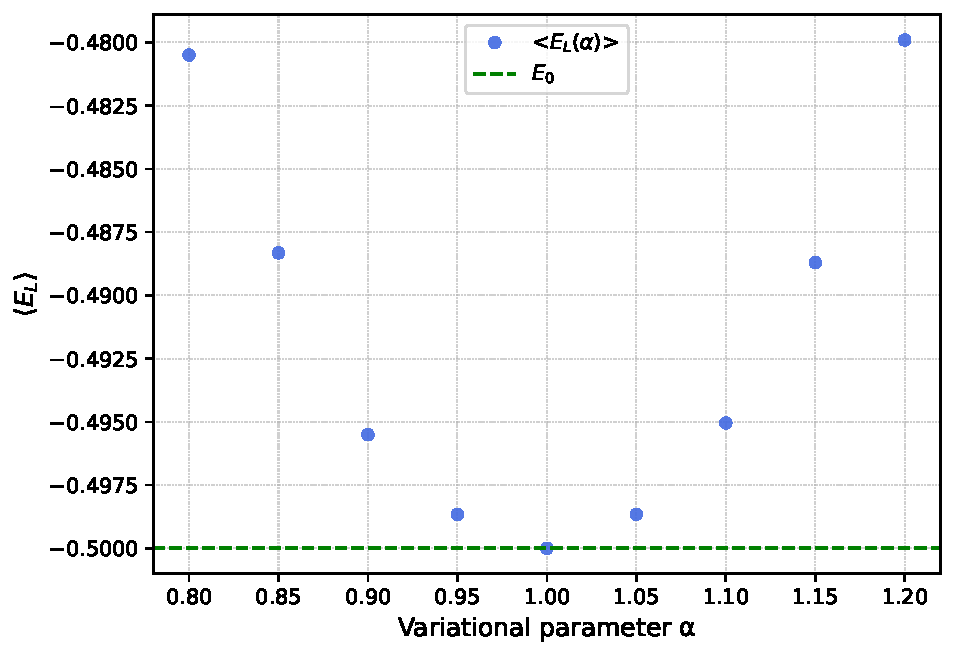
\includegraphics[width=\linewidth]{hydrogen.pdf}
            \caption{$\langle E_L \rangle$ over the full $\alpha$ grid, with the exact ground state energy $E_0 = -1/2$ as a reference. The x-axis shows the parameter $\alpha$ of the trial wavefunction $\psi_T$. The y-axis shows the expectation value calculated using the VMC approach.}
            \label{fig:hydrogen}
        \end{minipage}
    \end{figure}

    The exact wavefunction for hydrogen can also be calculated analytically and results in $\psi(r)) = e^{-|\vec{r}|}$, which is again part of the variational subspace as can be seen from the variance being 0 at the correct value of $\alpha=1$. It is obvious from the equations that through radial symmetry this could also have been calculated using just the 1 dimensional distance $|\vec{r}|$ but it was calculated in 3 dimensions for pedagogical purposes.

    \subsection{Helium atom}

    Helium introduces a second electron, which is described by the Hamiltonian

    \begin{equation}\label{eq:hamiltonian}
        H_{He} = -\frac{1}{2}\nabla_1^2 - \frac{1}{2}\nabla^2 - \
    \end{equation}

    \begin{table}[H]
        \centering
        \begin{tabular}{ccc}
\toprule
$\alpha$ & $\langle E \rangle$ & $\mathrm{var}(\langle E \rangle)$ \\
\midrule
$0.050$ & $-2.87074$ & $0.17567$ \\
$0.075$ & $-2.87514$ & $0.15368$ \\
$0.100$ & $-2.87706$ & $0.13634$ \\
$0.125$ & $-2.87782$ & $0.12241$ \\
$0.150$ & $-2.87820$ & $0.11202$ \\
$0.175$ & $-2.87804$ & $0.10339$ \\
$0.200$ & $-2.87716$ & $0.09684$ \\
$0.250$ & $-2.87397$ & $0.08865$ \\
\bottomrule
\end{tabular}

        \caption{VMC energies for the helium atom with the Jastrow-type trial wave function.}
        \label{tab:helium}
    \end{table}

    Improvements ...


    \printbibliography

%%% End document %%%
\end{document}